\documentclass[conference]{IEEEtran}

% The preceding line is only needed to identify funding in the first footnote. If that is unneeded, please comment it out.
\usepackage{cite}
\usepackage{amsmath,amssymb,amsfonts}
\usepackage{algorithmic}
\usepackage{graphicx}
\usepackage{textcomp}
\usepackage{xcolor}
\def\BibTeX{{\rm B\kern-.05em{\sc i\kern-.025em b}\kern-.08em
		T\kern-.1667em\lower.7ex\hbox{E}\kern-.125emX}}
\begin{document}
	
	\title{Progress Report: Intrusion Detection \\ 
		Leveraging Data Analytics and Machine Learning\\
		{\footnotesize \textsuperscript{*}}
		\thanks{Identify applicable funding agency here. If none, delete this.}
	}
	
	\author{\IEEEauthorblockN{1\textsuperscript{st} Kaung Sithu}
		\IEEEauthorblockA{\textit{department of Data Science and Artificial Intelligence} \\
			\textit{Asian Institute of Technology}\\
			Pathumthani, Thailand \\
			st124974@ait.asia}
		\and
		\IEEEauthorblockN{2\textsuperscript{nd} Mir Ali Taqi Nalpur}
		\IEEEauthorblockA{\textit{department of Data Science and Artificial Intelligence} \\
			\textit{Asian Institute of Technology}\\
			Pathumthani, Thailand \\
			st125001@ait.asia}
	}
	
	\maketitle
	
	\begin{abstract}
		This project addresses the limitations of traditional Intrusion Detection Systems (IDS) by developing a machine learning-based IDS using Intrusion Detection System datasets from the Canadian Institute for Cybersecurity. We apply algorithms such as Logistic Regression, Random Forest, and Deep Learning to classify network traffic and detect intrusions, including Denial of Service (DoS) attacks. Our approach involves data preprocessing, feature selection, and performance evaluation based on accuracy and F1-score. The results demonstrate that machine learning significantly enhances IDS effectiveness, offering a scalable solution for real-time network security.
	\end{abstract}
	
	\begin{IEEEkeywords}
		component, formatting, style, styling, insert
	\end{IEEEkeywords}
	
	\section{Progress Overview}
	\subsection{Data Selection}
	We selected the CIC-IDS dataset (including CIC-IDS17/18, DoS17, and DDoS19) due to its comprehensive and realistic network traffic data, which includes both benign and malicious network activities. This dataset is well-suited for intrusion detection, as it covers various types of attacks, such as DoS, DDoS, and more, providing a rich foundation for training and evaluating machine learning models. The inclusion of both attack and normal traffic types aligns with our goal of developing an effective and reliable intrusion detection system capable of identifying diverse cyber threats. 
	
	\subsection{Data Preprocessing}
	In our preprocessing pipeline, we performed several critical tasks to prepare the dataset for machine learning. We handled missing values appropriately, ensuring that no valuable data was discarded. We applied Min-Max scaling to normalize numerical features, which ensured that all features were on a similar scale and improved the model's performance. Feature selection was conducted to retain only the most relevant features, removing redundant or less informative ones. This step helped improve the dataset’s quality, ensuring that the machine learning models were trained on the most significant predictors.
	
	\subsection{Machine Learning Models}
	We included a variety of machine learning models to ensure robust evaluation of different approaches for the intrusion detection task. Specifically, we tested LightGBM, XGBoost, Naive Bayes, and SGDClassifier, each known for their strengths in classification tasks. By including multiple algorithms, we aimed to explore different model behaviors and select the best-performing one. Each model was fine-tuned using GridSearchCV to optimize hyperparameters, and a comparative analysis was conducted to determine which model provides the best performance for detecting network intrusions.
	
	\subsection{Performance Metrics}\label{AA}
	We included a variety of machine learning models to ensure robust evaluation of different approaches for the intrusion detection task. Specifically, we tested LightGBM, XGBoost, Naive Bayes, and SGDClassifier, each known for their strengths in classification tasks. By including multiple algorithms, we aimed to explore different model behaviors and select the best-performing one. Each model was fine-tuned using GridSearchCV to optimize hyperparameters, and a comparative analysis was conducted to determine which model provides the best performance for detecting network intrusions.
	
	\section{Detailed Progress}
	\subsection{Loading and Initial Inspection of Data}
	The dataset was loaded to inspect its structure, dimensions, and feature types, including various network traffic characteristics such as, packet sizes, connection durations, and protocols, as well as selecting the target variable, ClassLabel.
	
	\subsection{Feature Engineering and Selection}
	The dataset initially contained a wide range of features related to network traffic, such as packet lengths, flow durations, flags, and other network attributes. A correlation analysis was performed to identify and remove highly correlated features to avoid redundancy and multicollinearity, which could affect the model's performance. Features that were removed due to low and negative correlation include:
	\begin{itemize}
		\item Flow Duration
		\item Total Fwd Packets
		\item Total Backward Packets
		\item Fwd Packets Length Total
		\item Bwd Packets Length Total
		\item Fwd Packet Length Max
		\item Fwd Packet Length Mean
		\item Fwd Packet Length Std
		\item Bwd Packet Length Max
		\item Bwd Packet Length Mean
		\item Bwd Packet Length Std
		\item Flow Packets/s
		\item Flow IAT Mean'
		\item Flow IAT Std
		\item Flow IAT Max
		\item Flow IAT Min
		\item Fwd IAT Total
		\item Fwd IAT Mean
		\item Fwd IAT Std
		\item Fwd IAT Max
		\item Fwd IAT Min
		\item Bwd IAT Total
		\item Bwd IAT Mean
		\item Bwd IAT Std
		\item Bwd IAT Max
		\item Bwd IAT Min
		\item Fwd PSH Flags
		\item Fwd Header Length
		\item Bwd Header Length
		\item Fwd Packets/s
		\item Bwd Packets/s
		\item SYN Flag Count
		\item URG Flag Count
		\item Subflow Fwd Packets
		\item Subflow Fwd Bytes
		\item Subflow Bwd Packets
		\item Subflow Bwd Bytes		
		\item Init Fwd Win Bytes
		\item Init Bwd Win Bytes
		\item Fwd Act Data Packets
		\item Fwd Seg Size Min
		\item Active Mean
		\item Active Std
		\item Active Max
		\item Active Min
		\item Idle Mean
		\item Idle Std
		\item Idle Max
		\item Idle Min
	\end{itemize}
	
	\subsection{Final Set of Features}
	After performing correlation analysis and removing redundant features, the following features were retained for further analysis:
	\begin{itemize}
		\item Avg Packet Size
		\item Packet Length Mean
		\item Bwd Packet Length Std
		\item Packet Length Variance
		\item Bwd Packet Length Max
		\item Packet Length Max
		\item Packet Length Std
		\item Fwd Packet Length Mean
		\item Avg Fwd Segment Size
		\item Flow Bytes/s
		\item ClassLabel (target variable)
	\end{itemize}
	
	\subsection{Saving Preprocessed Dataframe}
	After preprocessing, the resulting DataFrame was saved to a parquet file. Thus, the processes such as cleaning, preprocessing and exploratory data analysis (EDA) are required not run on modeling notebook to save computation time and resources.
	
	\begin{figure}[h]
		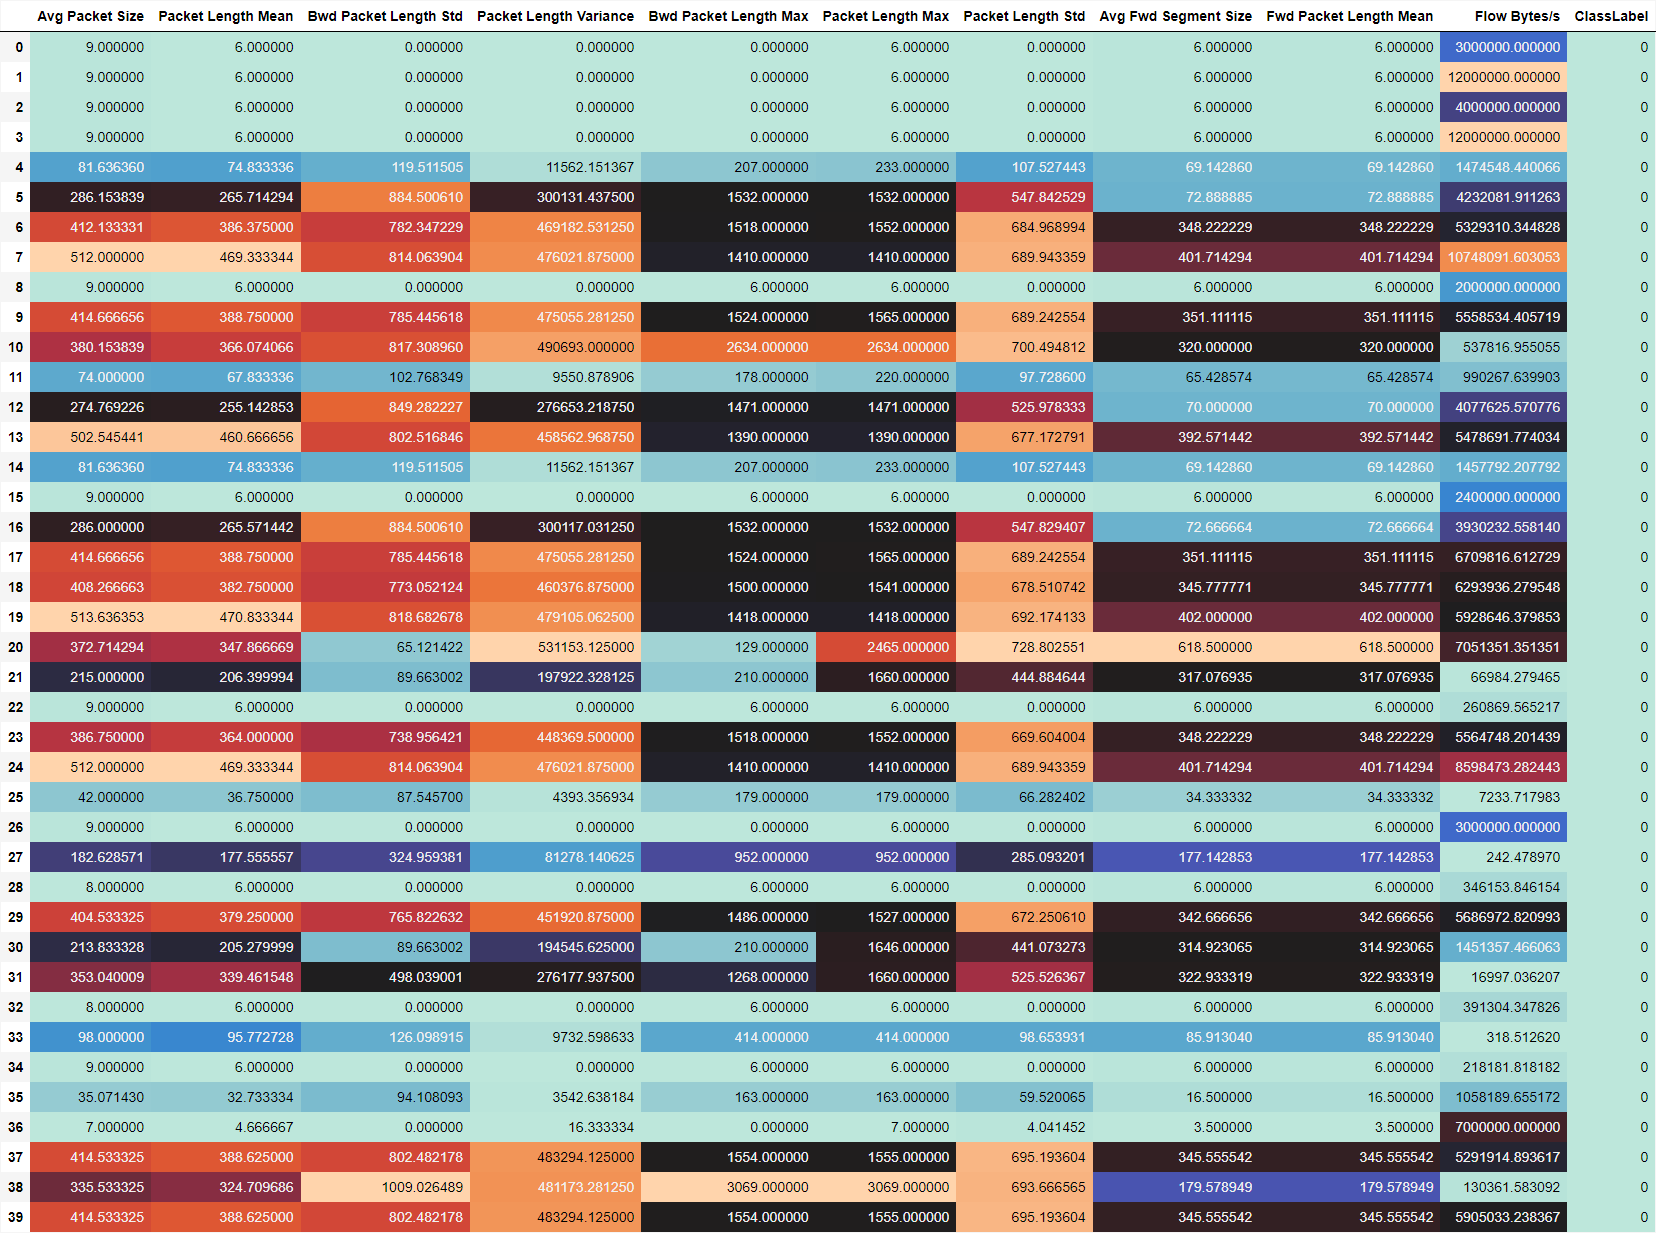
\includegraphics[width=\columnwidth]{my_df.png}
		\caption{First 40 rows of the dataset and all features}
	\end{figure}
	
	\subsection{Data Splitting}
	To prepare the dataset for model training and evaluation, we performed a train-test split. The dataset was divided into two subsets: a training set and a testing set. The training set contains the majority of the data and will be used to train the model, while the testing set will serve to evaluate the model's performance on unseen data.The features, which represent the various network traffic characteristics, were separated from the target variable, ClassLabel, which indicates whether the traffic is benign or associated with specific attack types. The data was split using a 70-30 ratio, where 70 percent of the data was allocated to the training set, and the remaining 30 was reserved for testing. The $train_test_split$ function from scikit-learn was used for this purpose, with a fixed random seed $(random_state=69)$ to ensure same results are produced each time the notebook is run. The shape of the splitted data are as follows:
	\begin{itemize}
		\item Training Features: 6,069,091 samples, 10 features
		\item Test Features: 2,601,039 samples, 10 features
		\item Training Labels: 6,069,091 samples
		\item Test Labels: 2,601,039 samples
	\end{itemize}
	This split ensures that the model is trained on a large portion of the data while being evaluated on a separate, hold-out set to assess its generalization capabilities.
	
	\subsection{Model Preparation and Configuration}
	To address the class imbalance and ensure effective model training, we applied several preprocessing and balancing techniques:
	\begin{itemize}
		\item Feature Scaling: \texttt{MinMaxScaler} was used to scale the numerical features in the dataset, transforming all numeric values to a range of [0, 1]. This ensures that no feature dominates due to its magnitude, which is especially important for models sensitive to feature scaling.
		\item Model Selection and Pipeline: The model pipeline was created using an \texttt{ImbPipeline} to integrate the preprocessing steps with the classification model. The classifier chosen for initial testing was \texttt{GaussianNB}, which is a simple and effective model for classification tasks. Additionally, other classifiers such as \texttt{LGBMClassifier}, \texttt{XGBClassifier}, and \texttt{SGDClassifier} were considered, with hyperparameters tuned through GridSearchCV.
		\item Parameter Grid for Model Tuning: A parameter grid for \texttt{GridSearchCV} was defined, allowing for the optimization of hyperparameters for different classifiers. The grid explored the following parameters:
		\subitem \texttt{LGBMClassifier}: num\_leaves, n\_estimators, and learning\_rate.
		\subitem \texttt{XGBClassifier}: max\_depth, n\_estimators, and learning\_rate.
		\subitem \texttt{SGDClassifier}: loss, alpha, penalty, and max\_iter.
	\end{itemize}
	
	This setup allows for a comprehensive evaluation of various models and hyperparameters to identify the best combination for effective classification of network traffic and attack detection.
	
	\subsection{Model Evaluation and Hyperparameter Tuning}
	To evaluate the performance of different classifiers and identify the optimal hyperparameters, we used GridSearchCV with cross-validation. The evaluation process consisted of the following steps:
	
	\begin{itemize}
		\item Stratified Cross-Validation: \texttt{StratifiedKFold} cross-validation strategy was employed, with 3 splits. This method ensures that each fold maintains the proportion of each class in the training and validation sets, providing more reliable performance metrics.
		\item GridSearchCV: \texttt{GridSearchCV} was set up to perform an exhaustive search over the hyperparameter grid. This search evaluated 20 different candidate configurations across 3 cross-validation folds, totaling 60 model fits. Macro F1 score was chosen as the evaluation metric to balance precision and recall across all classes, especially given the class imbalance.
		\item Best Model Parameters: After fitting the model, the best parameters were identified for the classifier. The best configuration found was for the \texttt{LGBMClassifier} with the following hyperparameters:
		\subitem Learning rate: 0.1
		\subitem Number of estimators: 50
		\subitem Number of leaves: 25
		
		These hyperparameters were selected to balance training time with model performance, ensuring optimal results for classifying network traffic. This grid search process helps identify the most effective classifier and hyperparameters, improving the model’s performance for intrusion detection tasks.
	\end{itemize}
	
	\subsection{Model Evaluation}
	After training the model using GridSearchCV with the LGBMClassifier, we evaluated its performance on the test dataset using classification metrics. The following key metrics were obtained:
	\begin{itemize}
		\item Overall Accuracy: The model achieved an accuracy of 87.65\% on the test set.
		\item Macro Average: Across all classes, the average precision, recall, and F1-score were 87.99\%, 95.83\%, and 90.01\%, respectively.
		\item Weighted Average: The weighted average F1-score was 89.02\%, taking into account the class imbalance.
	\end{itemize}
	Class-wise performance is as follows:
	\begin{itemize}
		\item Class 0 (e.g., Normal traffic): The model showed high precision (99.98\%) but lower recall (85.16\%), resulting in a balanced F1-score of 91.97\%.
		\item Class 1 (e.g., Specific attack type): The precision was slightly lower at 99.01\%, but the recall was high (98.76\%), yielding a very good F1-score of 98.89\%.
		\item Class 2: The model demonstrated excellent performance with precision of 99.36\%, recall of 99.51\%, and an F1-score of 99.43\%.
		\item This class had the lowest precision (53.59\%) due to the model predicting many false positives, though recall was nearly perfect at 99.91\%, resulting in an F1-score of 69.76\%.
	\end{itemize}
	These results suggest that the model performs exceptionally well on the majority of classes, especially in detecting specific attack types (Classes 1 and 2). However, there is room for improvement in Class 0 and Class 3, where recall and precision trade-offs could be better balanced.
	
\end{document}